%%%%%%%%%%%%%%%%%%%%%%%%%%%%%%%%%%%%%%%%%%%%%%%%%%%%%%%%%%%%%%%%%
%% 
%% IT Project Report template, v0.2
%% 
%% INSTRUCTIONS FOR COMPILING THIS DOCUMENT (using GNU/Linux command line)
%% 
%% pdflatex it-report.tex; bibtex it-report.aux
%% 
%%%%%%%%%%%%%%%%%%%%%%%%%%%%%%%%%%%%%%%%%%%%%%%%%%%%%%%%%%%%%%%%%

\documentclass[oneside,a4paper,11pt]{report}

%%%%%%%%%%%%%%%%%%%%%%%%%%%%%%%%%%%%%%%%%%%%%%%%%%%%%%%%%%%%%%%%%
%% PREAMBLE.
%%%%%%%%%%%%%%%%%%%%%%%%%%%%%%%%%%%%%%%%%%%%%%%%%%%%%%%%%%%%%%%%%

%%%%%%%%%%%%%%%%%%%%%%%%%%%%%%%%%%%%%%%%%%%%%%%%%%%%%%%%%%%%%%%%%
%% ANOTHER LATEX THESIS TEMPLATE.
%% https://github.com/zachscrivena/another-latex-thesis-template
%% This is free and unencumbered software released into the
%% public domain; see <http://unlicense.org> for details.
%%%%%%%%%%%%%%%%%%%%%%%%%%%%%%%%%%%%%%%%%%%%%%%%%%%%%%%%%%%%%%%%%



%%%%%%%%%%%%%%%%%%%%%%%%%%%%%%%%%%%%%%%%%%%%%%%%%%%%%%%%%%%%%%%%%
%% PAGE SIZE AND MARGINS.
%%%%%%%%%%%%%%%%%%%%%%%%%%%%%%%%%%%%%%%%%%%%%%%%%%%%%%%%%%%%%%%%%

% Letter-size (8.5in x 11in) single-sided pages,
% with margins (top,right,bottom,left) = (1,1,1,1.5)in,
% and header 0.25in above the text body.
\usepackage[
	paper=a4paper, % Default paper size, change to "letterpaper" for US Letter (you'll need to adjust margins after)
	inner=1.5in, % The inner margin (beside binding)
	outer=1in, % The outer margin (opposite binding)
	top=.8in, % Top margin
	bottom=.7in, % bottom margin
	headheight=20pt, % Header height
	headsep=.25in, % Header separation
	includehead,
	includefoot]{geometry}

%%%%%%%%%%%%%%%%%%%%%%%%%%%%%%%%%%%%%%%%%%%%%%%%%%%%%%%%%%%%%%%%%
%% COLORS.
%%%%%%%%%%%%%%%%%%%%%%%%%%%%%%%%%%%%%%%%%%%%%%%%%%%%%%%%%%%%%%%%%
\usepackage[usenames]{color} % For colors.

%%%%%%%%%%%%%%%%%%%%%%%%%%%%%%%%%%%%%%%%%%%%%%%%%%%%%%%%%%%%%%%%%
%% MISCELLANEOUS PACKAGES.
%%%%%%%%%%%%%%%%%%%%%%%%%%%%%%%%%%%%%%%%%%%%%%%%%%%%%%%%%%%%%%%%%

\usepackage{graphicx}
\usepackage[utf8]{inputenc}
\usepackage[english]{babel} % For language-specific hyphenation.
%\usepackage{polski}
\usepackage{cite} % Automatically sort and range citations numbers.
\usepackage{environ} % For easy definition of environments.
\usepackage{rotating} % For rotating objects.
\usepackage{framed} % For framed text.
\usepackage{enumitem}
\usepackage{longtable}
\usepackage{placeins}
\usepackage{lipsum}

%\hyphenation{dźwię-ku}

\usepackage{subfig}
\usepackage{tikz}
\usetikzlibrary{shapes,arrows,chains,decorations.markings,calc,shapes.geometric,intersections}
\usetikzlibrary{decorations.pathmorphing}
\usepackage{tkz-euclide}
%\usetkzobj{all}

\usepackage{longtable}
\usepackage{array}
\usepackage{multicol}
\newcommand{\inches}{$\mathrm{^{\prime\prime}}$}

\graphicspath{
	{Figures/}
	{./}
}

\newcommand{\todo}{\mbox{\color{red} TODO!}}



%%%%%%%%%%%%%%%%%%%%%%%%%%%%%%%%%%%%%%%%%%%%%%%%%%%%%%%%%%%%%%%%%
%% PDF OUTPUT.
%%%%%%%%%%%%%%%%%%%%%%%%%%%%%%%%%%%%%%%%%%%%%%%%%%%%%%%%%%%%%%%%%

% PDF settings and properties (set options with \hypersetup{}).
\usepackage{hyperref} % For TEX --> DVI --> PDF.
% \usepackage[pdftex]{hyperref} % For TEX --> PDF.

%%%%%%%%%%%%%%%%%%%%%%%%%%%%%%%%%%%%%%%%%%%%%%%%%%%%%%%%%%%%%%%%%
%% FONTS.
%%%%%%%%%%%%%%%%%%%%%%%%%%%%%%%%%%%%%%%%%%%%%%%%%%%%%%%%%%%%%%%%%

\usepackage[T1]{fontenc}
\usepackage{lmodern} % For Latin Modern fonts.
\usepackage{times}

% Sans-serif fonts.
\usepackage[scaled=0.89]{helvet}
\renewcommand{\sffamily}{\usefont{T1}{phv}{m}{n}}
\newcommand{\UseLMSSBoldFont}{\usefont{T1}{lmss}{m}{n}\bfseries}

% Monospace (typewriter) font.
\usepackage[scaled=0.78]{beramono}
\renewcommand{\ttfamily}{\usefont{T1}{fvm}{m}{n}}

%%%%%%%%%%%%%%%%%%%%%%%%%%%%%%%%%%%%%%%%%%%%%%%%%%%%%%%%%%%%%%%%%
%% SECTION HEADINGS.
%%%%%%%%%%%%%%%%%%%%%%%%%%%%%%%%%%%%%%%%%%%%%%%%%%%%%%%%%%%%%%%%%

% Section heading fonts.
\usepackage{sectsty} % For selecting fonts for section headings.
\allsectionsfont{\UseLMSSBoldFont}

% Section numbering depth.
\setcounter{secnumdepth}{10}

%%%%%%%%%%%%%%%%%%%%%%%%%%%%%%%%%%%%%%%%%%%%%%%%%%%%%%%%%%%%%%%%%
%% PARAGRAPHS.
%%%%%%%%%%%%%%%%%%%%%%%%%%%%%%%%%%%%%%%%%%%%%%%%%%%%%%%%%%%%%%%%%

% Line spacing.
\usepackage{setspace}
%\singlespacing
%\onehalfspacing
%\doublespacing
\setstretch{1.35} % custom

% Indented blocks.
\newcommand{\IndentBlock}[1]{\noindent\hangafter=0\hangindent=#1\parindent\ignorespaces}
\newcommand{\IndentHanging}{\noindent\hangafter=1\hangindent=\parindent\ignorespaces}

%%%%%%%%%%%%%%%%%%%%%%%%%%%%%%%%%%%%%%%%%%%%%%%%%%%%%%%%%%%%%%%%%
%% HEADERS AND FOOTERS.
%%%%%%%%%%%%%%%%%%%%%%%%%%%%%%%%%%%%%%%%%%%%%%%%%%%%%%%%%%%%%%%%%
% \includegraphics[height=0.5in]{ue.jpg}}
% Header.
\usepackage{fancyhdr}

\fancypagestyle{empty}{%
\fancyhf{}
\fancyhead[L]{\parbox[b]{20mm}{}}
\fancyhead[R]{\parbox[b]{48mm}{}}
\renewcommand{\headrulewidth}{0.0pt}
\renewcommand{\footrulewidth}{0.0pt}}

\fancypagestyle{regular}{%
\fancyhf{}
\fancyfoot[C]{\thepage}
\fancyhead[L]{\parbox[b]{20mm}{}}
\fancyhead[R]{\parbox[b]{48mm}{}}
\renewcommand{\headrulewidth}{0.0pt}
\renewcommand{\footrulewidth}{0.0pt}}

\fancypagestyle{plain}{%
\fancyhf{}
\fancyhead[L]{\parbox[b]{20mm}{}}
\fancyhead[R]{\parbox[b]{48mm}{}}
\fancyfoot[C]{\thepage}
\renewcommand{\headrulewidth}{0.0pt}
\renewcommand{\footrulewidth}{0.0pt}}

\pagestyle{regular}

%%%%%%%%%%%%%%%%%%%%%%%%%%%%%%%%%%%%%%%%%%%%%%%%%%%%%%%%%%%%%%%%%
%% FOOTNOTES.
%%%%%%%%%%%%%%%%%%%%%%%%%%%%%%%%%%%%%%%%%%%%%%%%%%%%%%%%%%%%%%%%%

% Blank footnotes.
\newcommand\BlankFootnote[1]{%
\begingroup%
\renewcommand{\thefootnote}{}%
\footnotetext{#1}%
\addtocounter{footnote}{-1}%
\addtocounter{Hfootnote}{-1}%
\endgroup}

%%%%%%%%%%%%%%%%%%%%%%%%%%%%%%%%%%%%%%%%%%%%%%%%%%%%%%%%%%%%%%%%%
%% LISTS.
%%%%%%%%%%%%%%%%%%%%%%%%%%%%%%%%%%%%%%%%%%%%%%%%%%%%%%%%%%%%%%%%%

% Numbered lists in IEEE style.
% (Individual lists can be modified by redefining
% these macros inside the enumerate environment.)
\makeatletter
% 1st level: 1), 2), 3)
\renewcommand{\theenumi}{\arabic{enumi}}
\renewcommand{\labelenumi}{\theenumi)}
% 2nd level: a), b), c)
\renewcommand{\theenumii}{\alph{enumii}}
\renewcommand{\labelenumii}{\theenumii)}
\renewcommand\p@enumii{}
% 3rd level: i), ii), iii)
\renewcommand{\theenumiii}{\roman{enumiii}}
\renewcommand{\labelenumiii}{\theenumiii)}
\renewcommand\p@enumiii{}
% 4th level: A), B), C)
\renewcommand{\theenumiv}{\Alph{enumiv}}
\renewcommand{\labelenumiv}{\theenumiv)}
\renewcommand\p@enumiv{}
\makeatother

% Definition items.
\newcommand{\DefineItem}[1]{%
\IndentBlock{1}#1\nopagebreak
\par\IndentBlock{2}}


%%%%%%%%%%%%%%%%%%%%%%%%%%%%%%%%%%%%%%%%%%%%%%%%%%%%%%%%%%%%%%%%%
%% FIGURES AND TABLES.
%%%%%%%%%%%%%%%%%%%%%%%%%%%%%%%%%%%%%%%%%%%%%%%%%%%%%%%%%%%%%%%%%

\usepackage{graphicx} % To support graphics in EPS format.
\usepackage{multirow} % To support multi-row cells in tables.
\usepackage{booktabs} % For making nice tables.

% Adjust spacing between table rows.
\renewcommand*\arraystretch{1.25}

% Dashed lines in tables.
\usepackage{arydshln}
\def\dashvertical{;{2pt/3pt}}
\def\dashhorizontal{\hdashline[2pt/3pt]}

% Captions for figures and tables.
\newcommand{\CaptionFontSize}{\small}

\makeatletter
\def\@figurestring{figure}
\def\@tablestring{table}
\def\@makecaption#1#2{%
\CaptionFontSize
\ifx\@captype\@figurestring
\vskip1em
\fi
\sbox\@tempboxa{{\sffamily\bfseries{#1.}}\hspace{0.5em}#2}%
\ifdim\wd\@tempboxa>\hsize
{{\sffamily\bfseries{#1.}}\hspace{0.5em}#2}%
\else
\hb@xt@\hsize{\hfil\box\@tempboxa\hfil}%
\fi
\ifx\@captype\@tablestring
\vskip1em
\fi
}
\makeatother


%% \definecolor{MyDarkBlue}{rgb}{0,0.08,0.45}
%% {\color{MyDarkBlue}This text is dark blue}

%%%%%%%%%%%%%%%%%%%%%%%%%%%%%%%%%%%%%%%%%%%%%%%%%%%%%%%%%%%%%%%%%
%% DATE AND TIME.
%%%%%%%%%%%%%%%%%%%%%%%%%%%%%%%%%%%%%%%%%%%%%%%%%%%%%%%%%%%%%%%%%

\usepackage{datetime} % For dates and times.
\renewcommand{\dateseparator}{-}
\settimeformat{xxivtime}

% Timestamp.
\newcommand{\Timestamp}{{\yyyymmdddate\today}~{\currenttime}}


%%%%%%%%%%%%%%%%%%%%%%%%%%%%%%%%%%%%%%%%%%%%%%%%%%%%%%%%%%%%%%%%%
%% MATHEMATICS.
%%%%%%%%%%%%%%%%%%%%%%%%%%%%%%%%%%%%%%%%%%%%%%%%%%%%%%%%%%%%%%%%%

\usepackage{amsmath,amsfonts,amsbsy,amsthm} % AMS packages.



%%%%%%%%%%%%%%%%%%%%%%%%%%%%%%%%%%%%%%%%%%%%%%%%%%%%%%%%%%%%%%%%%
%% TABLE OF CONTENTS (TOC) SETTINGS.
%%%%%%%%%%%%%%%%%%%%%%%%%%%%%%%%%%%%%%%%%%%%%%%%%%%%%%%%%%%%%%%%%

% TOC depth.
\setcounter{tocdepth}{10}

% Suppress entries in the TOC.
\newcommand{\DummyThree}[3]{}

\newcommand{\DisableTOCUpdates}{%
\let\tempaddcontentsline=\addcontentsline
\let\addcontentsline=\DummyThree}

\newcommand{\EnableTOCUpdates}{%
\let\addcontentsline=\tempaddcontentsline}


\usepackage{lipsum} % For sample/blind text.





%%%%%%%%%%%%%%%%%%%%%%%%%%%%%%%%%%%%%%%%%%%%%%%%%%%%%%%%%%%%%%%%%
%% ACTUAL DOCUMENT.
%%%%%%%%%%%%%%%%%%%%%%%%%%%%%%%%%%%%%%%%%%%%%%%%%%%%%%%%%%%%%%%%%

\begin{document}

% Use Roman numerals (i, ii, iii, etc.) for page numbers.
\pagenumbering{roman}

%%%%%%%%%%%%%%%%%%%%%%%%%%%%%%%%%%%%%%%%%%%%%%%%%%%%%%%%%%%%%%%%%
%% TITLE PAGE.
%%%%%%%%%%%%%%%%%%%%%%%%%%%%%%%%%%%%%%%%%%%%%%%%%%%%%%%%%%%%%%%%%

% No headers or footers on the title page.
\thispagestyle{empty}

\begin{titlepage}
{\centering
\setstretch{1.0}
\null
\vspace{-1.0in}

\includegraphics[width=1.8in]{polsl_logo2_zn_en.pdf}\\[2.5em]
\normalfont\LARGE
Faculty of Automatic Control, \\Electronics and Computer Science \\[1.3em]
\normalfont\LARGE
Internet Technologies -- project work \\[1.5em]
\UseLMSSBoldFont\LARGE
WebPage with charts\\[5.2em]}
\normalfont\large
\noindent
Authors: 
\\[0.5em]
Michał Siedlaczek
\\[1.5em]
2021, 5, 2, 2: 
\\[0.5em]
Project supervisor: dr inż. Stanisław Wrona
\\[1.5em]

\vfill
\centering Gliwice 2021
\par
\end{titlepage}




\pagestyle{plain}
\setcounter{page}{2}


\clearpage



%%%%%%%%%%%%%%%%%%%%%%%%%%%%%%%%%%%%%%%%%%%%%%%%%%%%%%%%%%%%%%%%%
%% TABLE OF CONTENTS (TOC), LISTS OF FIGURES/TABLES/ETC.
%%%%%%%%%%%%%%%%%%%%%%%%%%%%%%%%%%%%%%%%%%%%%%%%%%%%%%%%%%%%%%%%%

\tableofcontents

%\listoffigures

%\listoftables

\clearpage


% Use Arabic numerals (1, 2, 3, etc.) for page numbers.
\pagenumbering{arabic}




\chapter{Introduction}

%\lipsum[1] Logo uczelni pokazane jest na Fig. \ref{fig:logo}.

The Internet is a worldwide collection of computer networks that began as a single network that was originally created in 1969 by ARPA (Advanced Research Projects Agency), a U.S. government agency that was far more interested in creating projects that would survive a nuclear war than in creating anything useful for the civilian population.

In its original form, ARPANET, the U.S. government hoped to create a network of computers that would allow communication between government agencies and certain educational centers that would be able to survive a nuclear explosion. It is doubtful that the original founders of ARPANET foresaw what we now know as "the Internet." From its humble beginnings as a military project, the ARPANET grew slowly throughout the 70's and 80's as a community of academics accomplished the truly monumental task of hammering out the building blocks of this new, open, modular conglomeration of networks.

In addition to the U.S. ARPANET, other countries also developed their own computer networks which quickly linked up to ARPANET, such as the UK's JANET (1983 onwards), and Australia's ACSnet (mid-1970s until replaced). Connecting these together would help develop a global internetwork.

The various protocols, including IP, TCP, DNS, POP, and SMTP, took shape over the years, and by the time the World Wide Web (HTML and HTTP) was created in the early 90's, this "Internet" had become a fully functional, fairly robust system of network communication, able to support this new pair of protocols which eventually turned the Internet into a household word.

While a large portion of users today confuse the Web with the Internet itself, it must be emphasized that the Web is only one type of Internet application, and one set of protocols among a great many which were in use for over a decade before the Web entered into the public awareness.


%\cite{wikipedia}.

Odnosnik \cite{wikipedia}.

%\begin{figure}
%	\centering
%	
\includegraphics[width=1.7in]{polsl_logo2_zn_en.pdf}
%	\caption{To jest logo.\label{fig:logo}}
%\end{figure}
	
%\lipsum[3-7] 


\chapter{Aim and scope of the project}
The main goal of my project is to create a website that will allow to analyze data in easy way. A website will display charts which gives us data about velocity and distance traveled as a function of time.
The page should has a menu where we can choose velocity char, distance traveled chart, blog or contact. I want to use programming languages C, PHP, JavaScript and markup language HTML, CSS. Also after finish the project i want use bootstrap to make a page compatible with other devices.

Project assumptions:\newline
1.Learn the basics. How to program in html, css, javascript, php.\newline
2.Make simple WebPage with charts.\newline
3.Project allows us to understand networks and servers.\newline
4.Project allows to gain experience with solving problems.\newline
5.Learn how to write report in latex.\newline
6.Gives us experience in html, css, javascript etc. that we can program in frameworks.\newline
7.Learn technical english and how to use it. Preparing to work with english language. \newline
\begin{figure}
	\centering
	
\includegraphics[width=2.7in]{itzdjecie.jpg}
	\caption{Goal and idea.\label{fig:Goal and Idea}}
\end{figure}
\chapter{Schedule}
\section{Schedule approved at the beginning}
8.01 Learn the basics. How to program simple things. Create page or application without anything on it. \newline
15.01 Send data to my page or application and create charts with this data.\newline
22.01 Solve problems, upgrade your page, add some text to give information about page. \newline
\section{Schedule reflecting actual work}
I did all things i want to and which i have in approved schedule, but i didn't manage to make properly work server with arduino which sends data to database. In future i want repair this problems and try webpage with bootstrap.
\begin{figure}
	\centering
	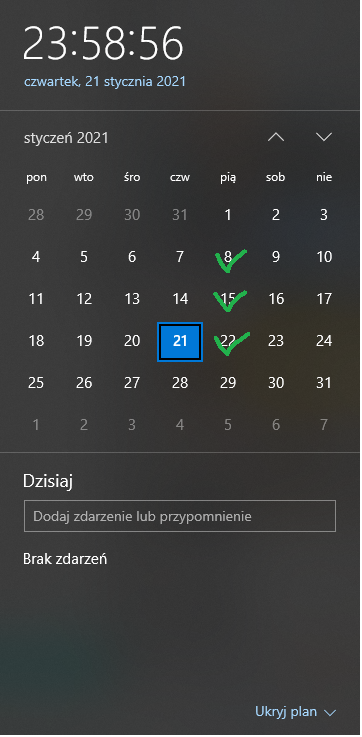
\includegraphics[width=1.0in]{schedule.png}
	\caption{Schedule.\label{fig:Schedule}}
\end{figure}
\chapter{Software and/or hardware implementation WebPage with charts}
\section{Defining the problem}
How we can do the WebPage? We can do it with standard languages or extensive frameworks like for example Angular. Firstly i thought about do html, css files which i need to create my WebPage. WebPage can exist because html files. Css files are for better look of the webpage. I thought about how my webpage will look like. I created html and css files and wrote lines of code in this files. Secondly i thought about elements which i must buy to send data from arduino sensors to database. I bought ArduCam with esp inside it, but something wasn't working, so then i bought Ethernet-Shield. Then i thought how to implement code in arduino environment. I didn't manage to properly implement it to send data from sensors by ethernet shield. In future i will try again or do it by python. After it i created javascript files and php files. Javascript files cause drawing charts and php files cause connect database with my webpage. 
\begin{figure}
	\centering
	
\includegraphics[width=2.0in]{okreslicproblem.jpeg}
	\caption{Defining the problem.\label{fig:Defining the problem}}
\end{figure}

\section{Analysis of possible solutions}
To do html files the solution is just to write adequate code in html language. To do that I must learn bacics of html with guides on youtube or google. How will my page look like? How to solve this problem? It is good question. To do that I must learn bacics of html with guides on youtube or google. Firstly i think it is good to draw idea on paper and calculate everything. Then try to program our idea in css files. Also we must do diffrent css files to diffrent html files. We could change html files with php files to not changing all html files or save content of all subpages to database. \newline
How can I do WebServer? I can do it with arduino, python or just try free hosting on internet. \newline How can I send data from arduino to my WebPage? Firstly i must learn how to implement code in arduino to send data and buy required items. Then i must learn php files which will help me to receive the data from arduino and send data from database to my webpage. I think it can work with only arduino code in which is html code etc.\newline 
\section{The proposed solution}
I chose basic programming like html, css, javascript, php and of course C on arduino. I chose it because I could find really good guides on youtube-pasja informatyki and a lot of other video stuff with creating charts with javascript libaries. It is diffucult to learn something like angular or something without know the basics. Also it is smaller amount of guides because it is hard to master something, lets say big amount of programming. \newline
\newline
I thought about sending data from arduino to WebPage but finally i did it with database which i think is better. Data is send from arduino to database and then WebPage receive this data from database and create charts.\newline
I did my WebPage with a lot of htmls, css, javascript, php files which isn't that good,although it is ok, could be better with database, but there was small amount of time to do that project. 


\frac{dQ}{dt}=Q_{in}-Q_{out}+P\\
\frac{dV\cdot\rho \cdot c_{w}}{dt}=F\cdot \rho \cdot c_w \cdot T_{in}-F\cdot \rho\cdot c_w\cdot T_{out}+P\\
\frac{dT_{out}}{dt}=\frac{F}{V}\cdot(T_{in}- T_{out})+\frac{1}{V\cdot \rho \cdot c_w}\cdot P\\
K(s)=\frac{\Delta T_{out}}{\Delta P}=\frac{\frac{1}{V\cdot \rho \cdot c_w}\cdot\frac{V}{F}}{\frac{V}{F}s+1}\\
G=\frac{1}{V\cdot \rho \cdot c_w}\cdot\frac{V}{F}\\
\tau=\frac{V}{F}//
\section{Implementation}
Arduino Implementation:\newline
Initialize the Ethernet server library with port:\newline
EthernetServer server(80);\newline
How to set up IP address for my controller:\newline
IPAddress ip(192, 168, 0, 137);\newline
Start the Ethernet connection and the server:\newline
Ethernet.begin(mac, ip);\newline
Listen for incoming clients:\newline
EthernetClient client=server.available();\newline
\newline
\newline
We check connection with:\newline
if(client.connected())\newline
And then arduino sends request to a server with:\newline
client.print("GET /testcode/rower.php?v2=");\newline
client.print(v2);\newline
client.print("ANDprzebytadroga=");\newline %and&
client.print(przebytadroga);\newline
Standard http response header\newline
client.print(" ");\newline
client.print("HTTP/1.1");\newline
client.println();\newline
client.println("Connection: close");\newline
client.println();\newline
\newline
\newline
Html Implementation:\newline
Standard code need:\newline
<html></html>\newline
<body></body>\newline
<head></head>\newline
<!DOCTYPE HTML>\newline
<html lang="pl">\newline
<meta charset="utf-8"/>\newline
\newline
Css Implementation:\newline
We can add background by:\newline
body\newline
nawiasklamrowy\newline
	background-image:url('rower.jpg');\newline
	background-size:cover;\newline
	background-position:center;\newline
	position:relative;\newline
	overflow:hidden;\newline
nawiasklamrowy\newline
\newline
We should add Id by hashtag or class by dot. Then in id or class we should write width, height, color, text-allign, padding, background-color, font-size and other stuff. For example:\newline
hashtagwstep\newline
nawiasklamrowy\newline
	background-color:black;\newline
	color:black;\newline
	text-align:center;\newline
	padding: 15px;\newline
	letter-spacing: 2px;\newline
nawiasklamrowy\newline
\newline
The float command is usefull. The float CSS property places an element on the left or right side of its container, allowing text and inline elements to wrap around it. \newline
Also to clear float command we need to use clear:both.\newline
Creating charts:\newline
You need to create a php file that will connect to the database and retrieve data using:\newline
mysqli = new mysqli(DBHOST, DBUSERNAME, DBPASSWORD, DBNAME); with dollar at the beginning of course\newline
query = sprintf("SELECT v2, przebytadroga FROM rower"); with dollar at the beginning of course\newline
\newline
\newline
Also we need to create a javascript files. In it, the push() method adds more points to the array. Using the get method we download the php url file.
To create a chart, we need to create an instance of the Chart class with:\newline
<canvas id = "mycanvas" width = "400" height = "400"> </canvas>\newline
var ctx =  ("mycanvas");with dollar after equal symbol of course and hashtag before mycanvas\newline


We need to create an html file in which we need to include the appropriate files from javascript:\newline
<script type="text/javascript" src="js/jquery.min.js"></script>\newline
<script type="text/javascript" src="js/Chart.min.js"></script>\newline
<script type="text/javascript" src="js/app1.js"></script>\newline
\newline

\section{Problems during project development}
As always, there are problems with any project. In this project there were problems too.\newline The main problems was to implement the code and working properly.\newline First problem was to how implement graphic in website, but it is easy to solve, but sometimes i had problems with css files, where i saved this and nothing happens. \ref{fig:Css} \newline \newline
Secondly my ArduCam ESP8266-12E WiFi IoT didn't work i didn't know why, so i changed to ethernet shield. Then Ethernet shields need to use some of pins to work properly. The Ethernet shield uses digital pins 11, 12, 13, 10, and 4 for SPI communication, so i couldn't connect my lcddisplay and other stuff: rtc, buttons. Even simple program like "Hello world" didn't want display on lcd. When i changed to analog my program didn't want calculate, so i just removed lcd and other stuff to make project easier. \ref{fig:Esbp} \newline \newline \newline
To create server was a problem too. Probably the problem was in library i used which is ethernet.h then i changed it to ethernet2.h, and i had server but it didn't send data to database I didn't figure out why. \ref{fig:Server}\newline \newline
\begin{figure}[!b]
	\centering
	
\includegraphics[width=5.0in]{css.png}
	\caption{Css.\label{fig:Css}}
\end{figure}

\begin{figure}[!b]
	\centering
	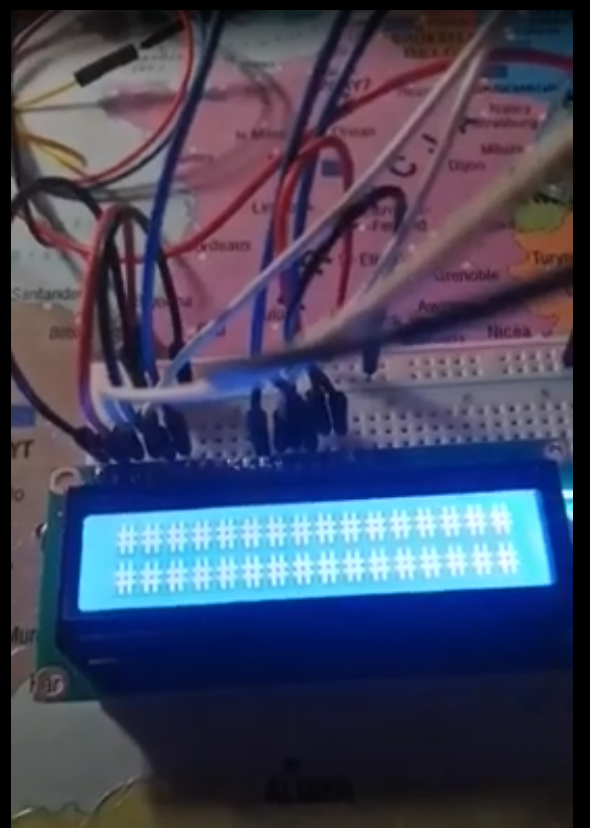
\includegraphics[width=2.7in]{esbp.png}
	\caption{Ethernet Shield pins problem.\label{fig:Esbp}}
\end{figure}

\begin{figure}[!b]
	\centering
	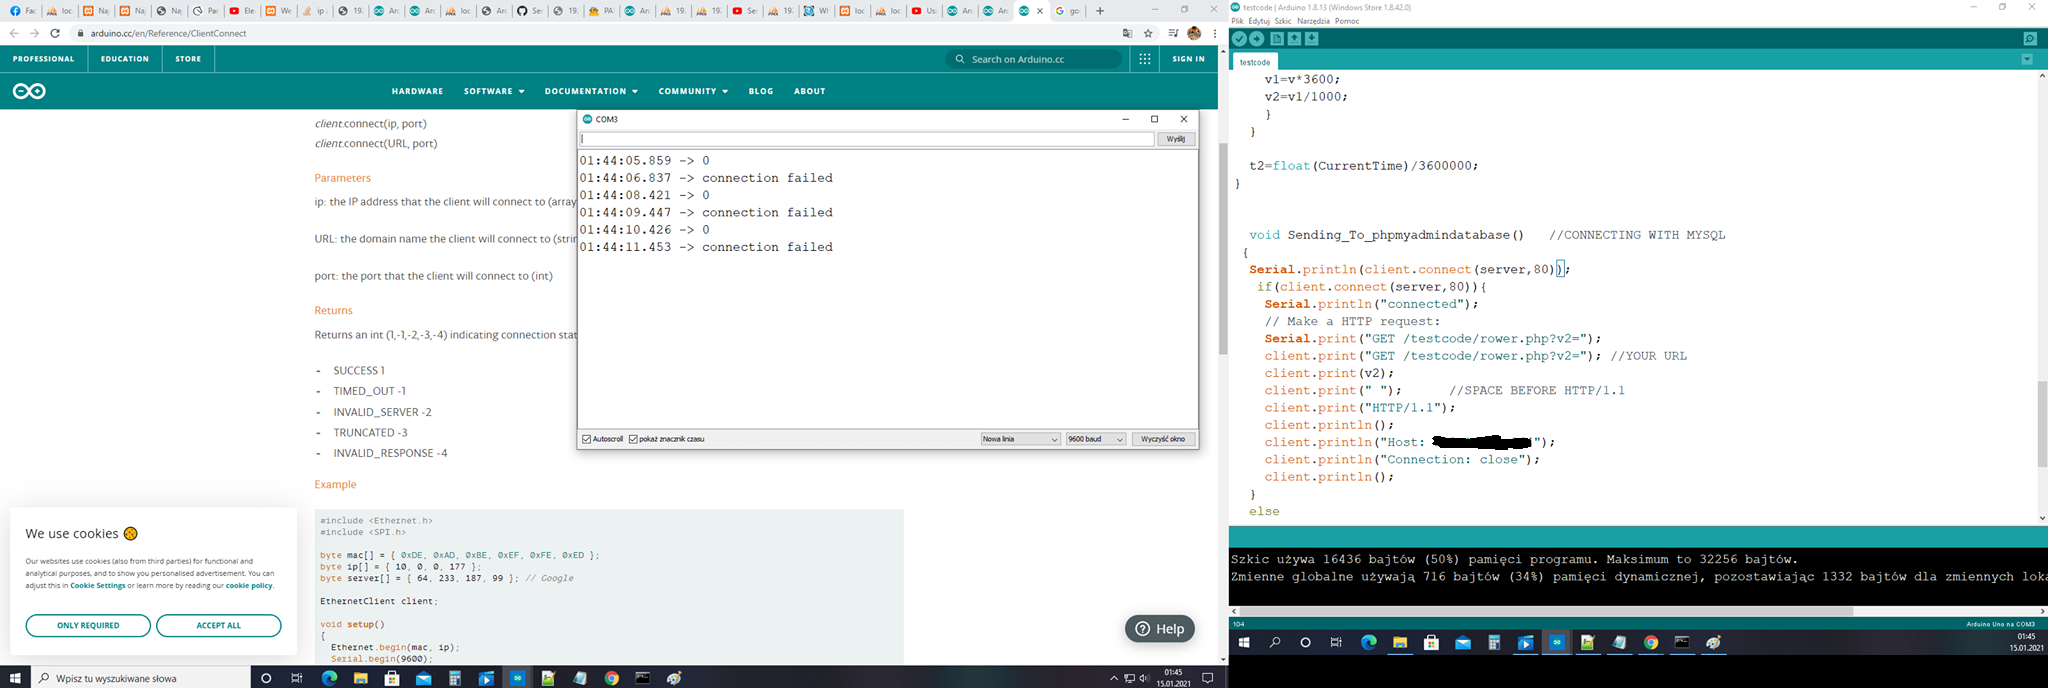
\includegraphics[width=5.0in]{server.png}
	\caption{Server problem.\label{fig:Server}}
\end{figure}
\chapter{Summary}
Price of the project!
It depends where u buy arduino, ethernet shields etc. If i didn't add project from other lesson it could be around from 70PLN to 170PLN depends on which website u will buy or in what store. Also the price is the time you have to learn many languages.
\begin{figure}[!h]
	\centering
	
\includegraphics[width=2.5in]{cena.jpg}
	\caption{Price.\label{fig:Cena}}
\end{figure}
\newline
\newline
I gained the ability to program in various languages, to program in markup languages, i.e. html and css, to create graphs on a website with the help of data retrieval from a database.

\begin{figure}[!h]
	\centering
	
\includegraphics[width=2.5in]{skill.png}
	\caption{Skill.\label{fig:Skill}}
\end{figure}
What's next?\newline
1. To fix not working properly server.\newline
2. Maybe do it with only arduino without database.\newline
3. Add some animation on page.\newline
4. Add some other charts maybe do it with real time chart with showing only 20 data points.\newline
5. Improve the website so that it can be used from various devices on the internet.\newline
\newline
\newline
To sum up i learnt a lot of things. I learnt how to program in different languages. Also I gain knowledge to do my project or knowledge useless to my project but maybe usefull in future. Also I improved english skills with writing a raport and making a presentation, I improved my english speach. I learnt how to send data from arduino to database and from database to WebPage. I improved my skills with database. I got experience in making charts on webpages. It was really fun to do the project. Now I have more knowledge and can do other projects or improve my WebPage to better stage.
\begin{figure}[!b]
	\centering
	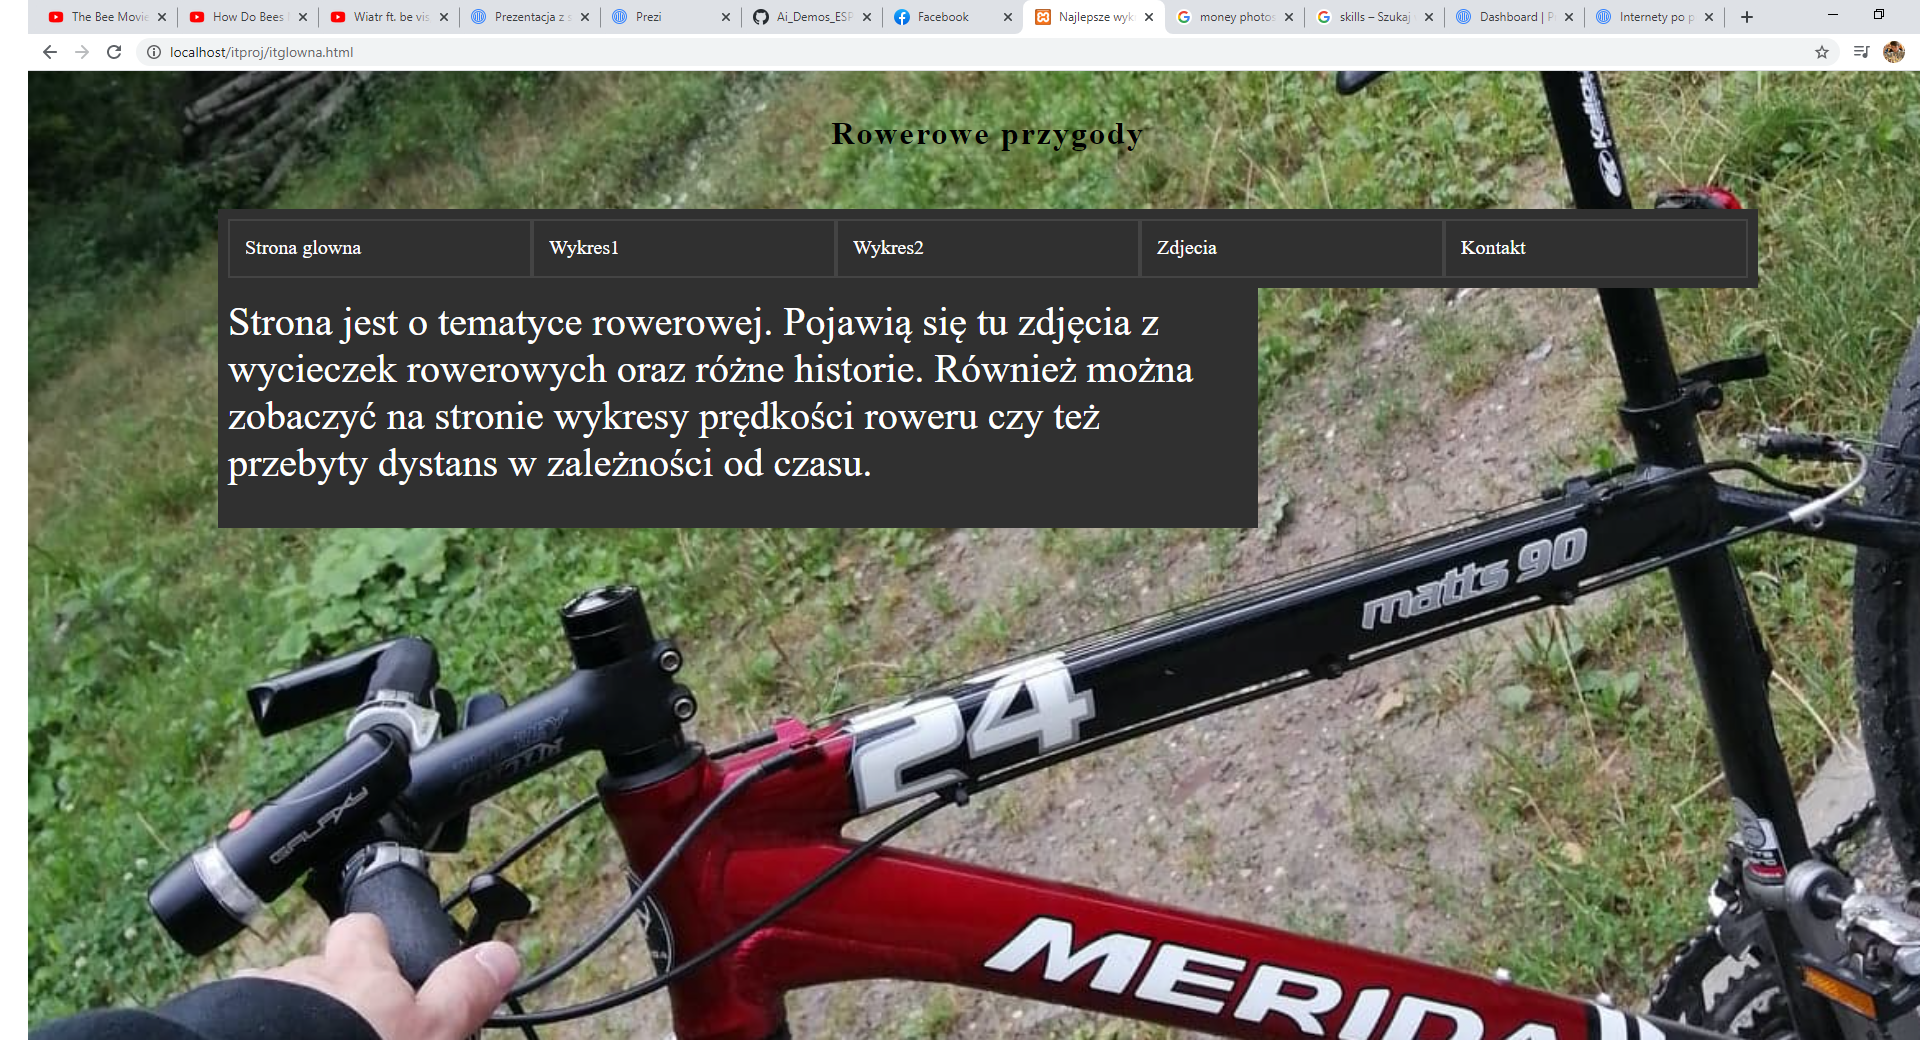
\includegraphics[width=5.0in]{stronaglowna.png}
	\caption{Moja Strona.\label{fig:Stronaglowna}}
\end{figure}
\newline
On the end i can add photo with my arduino and how arduCam with build esp in it look like.\newline

\begin{figure}[!b]
	\centering
	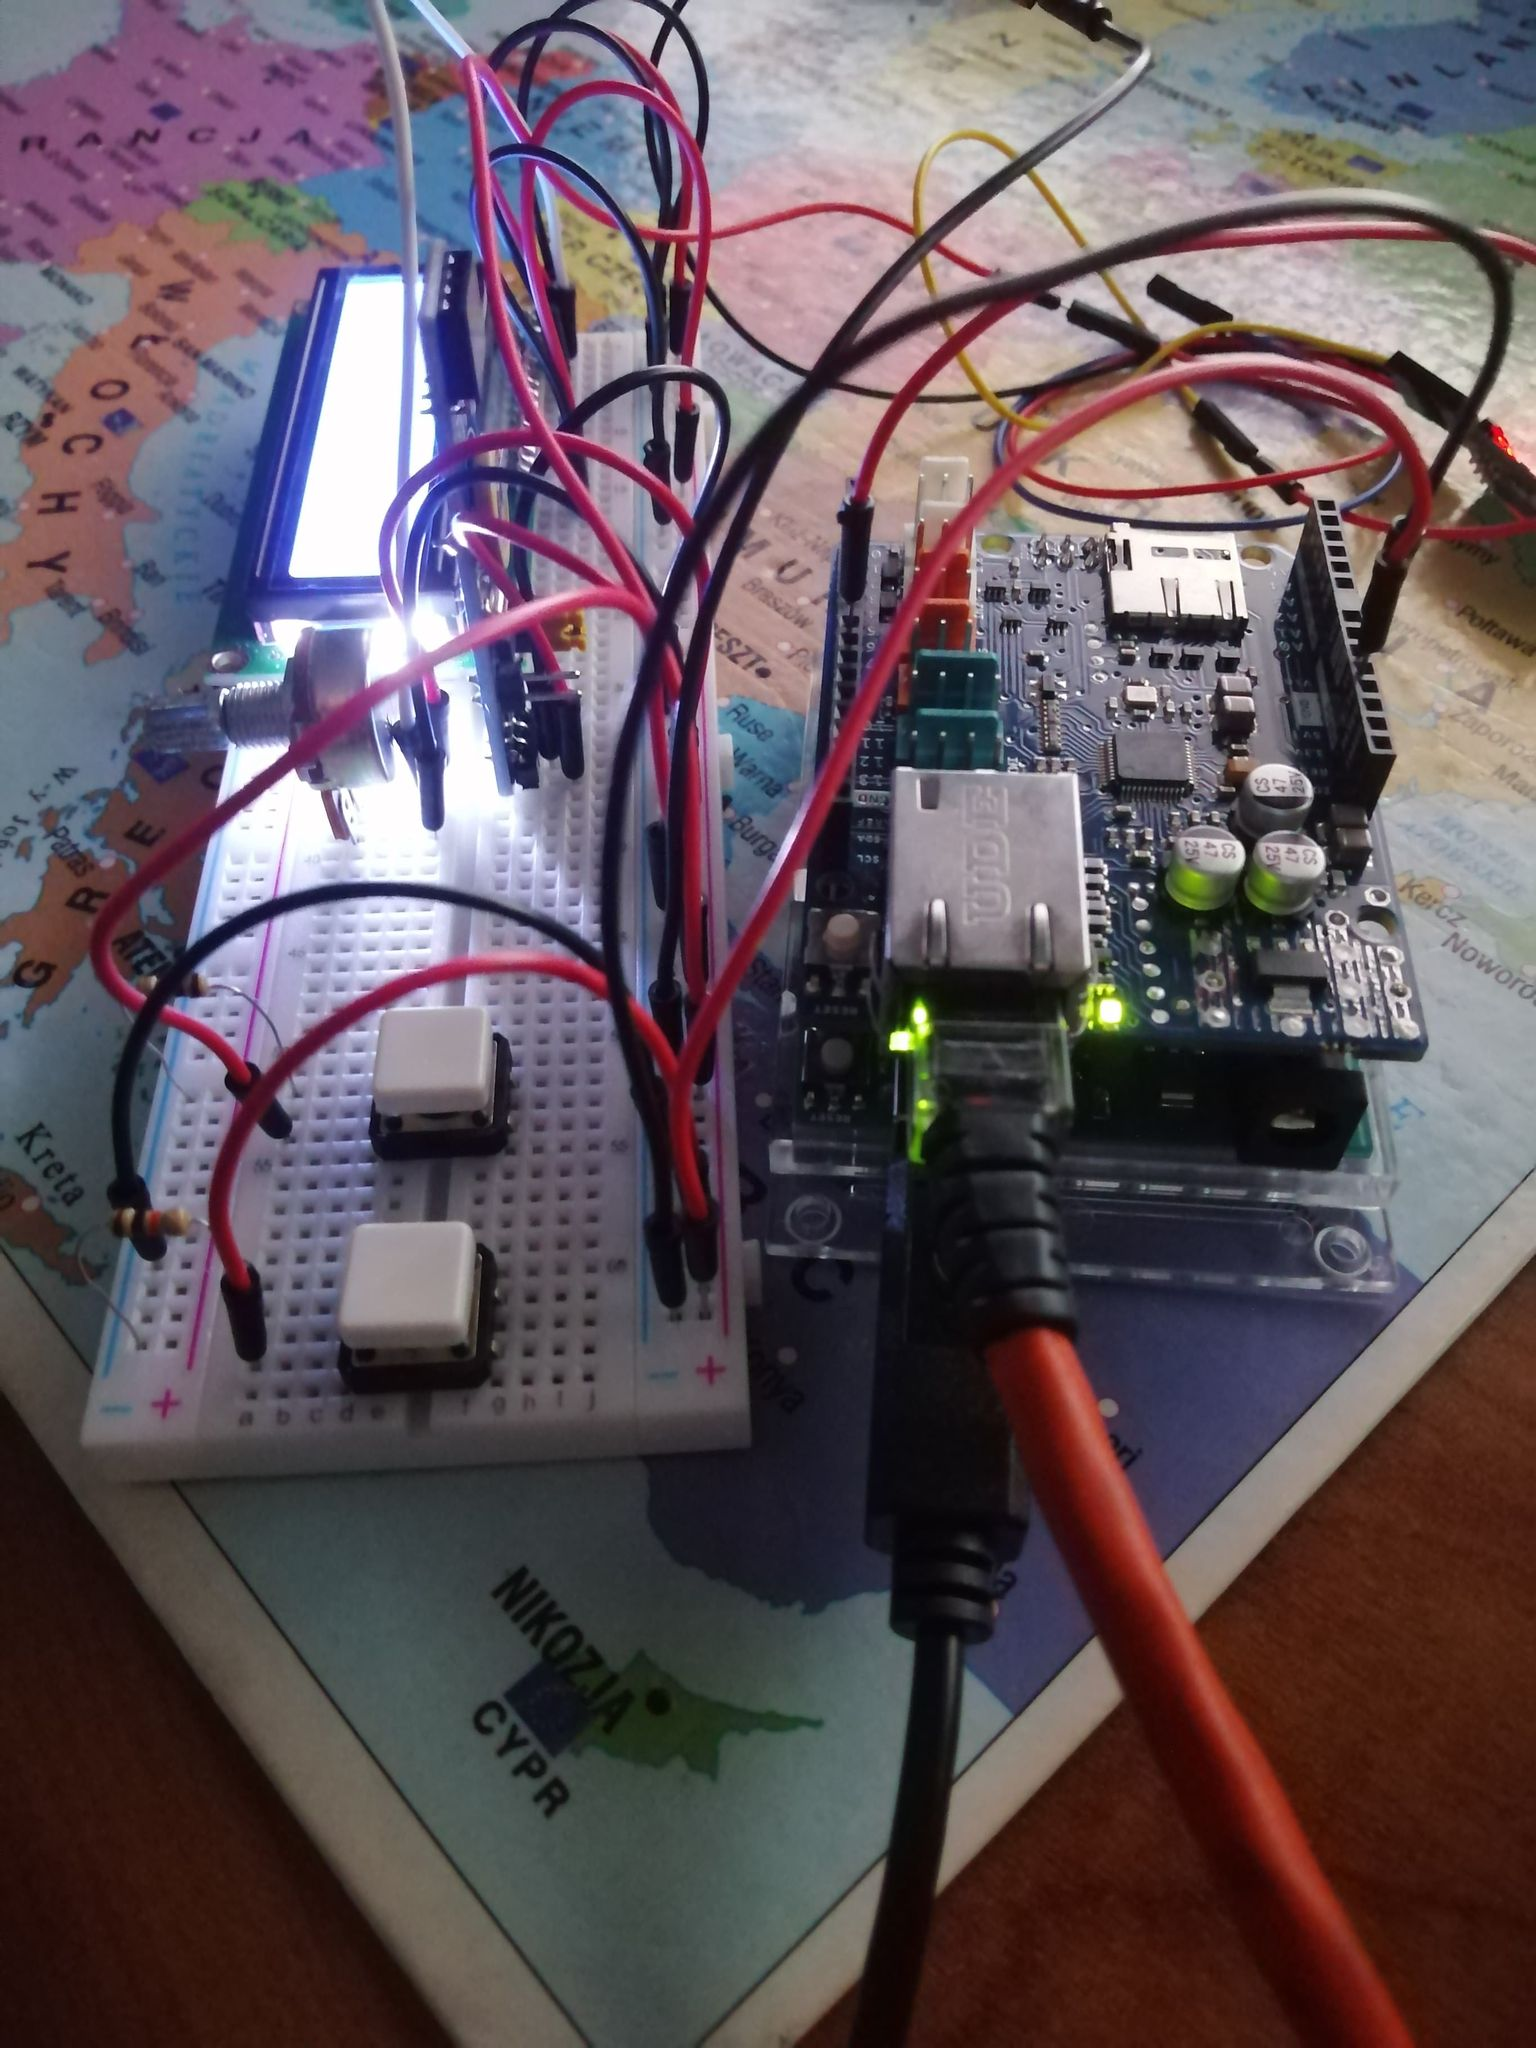
\includegraphics[width=5.0in]{mojuklad.jpg}
	\caption{My arrangement.\label{fig:Myarrangement}}
\end{figure}
\begin{figure}[!b]
	\centering
	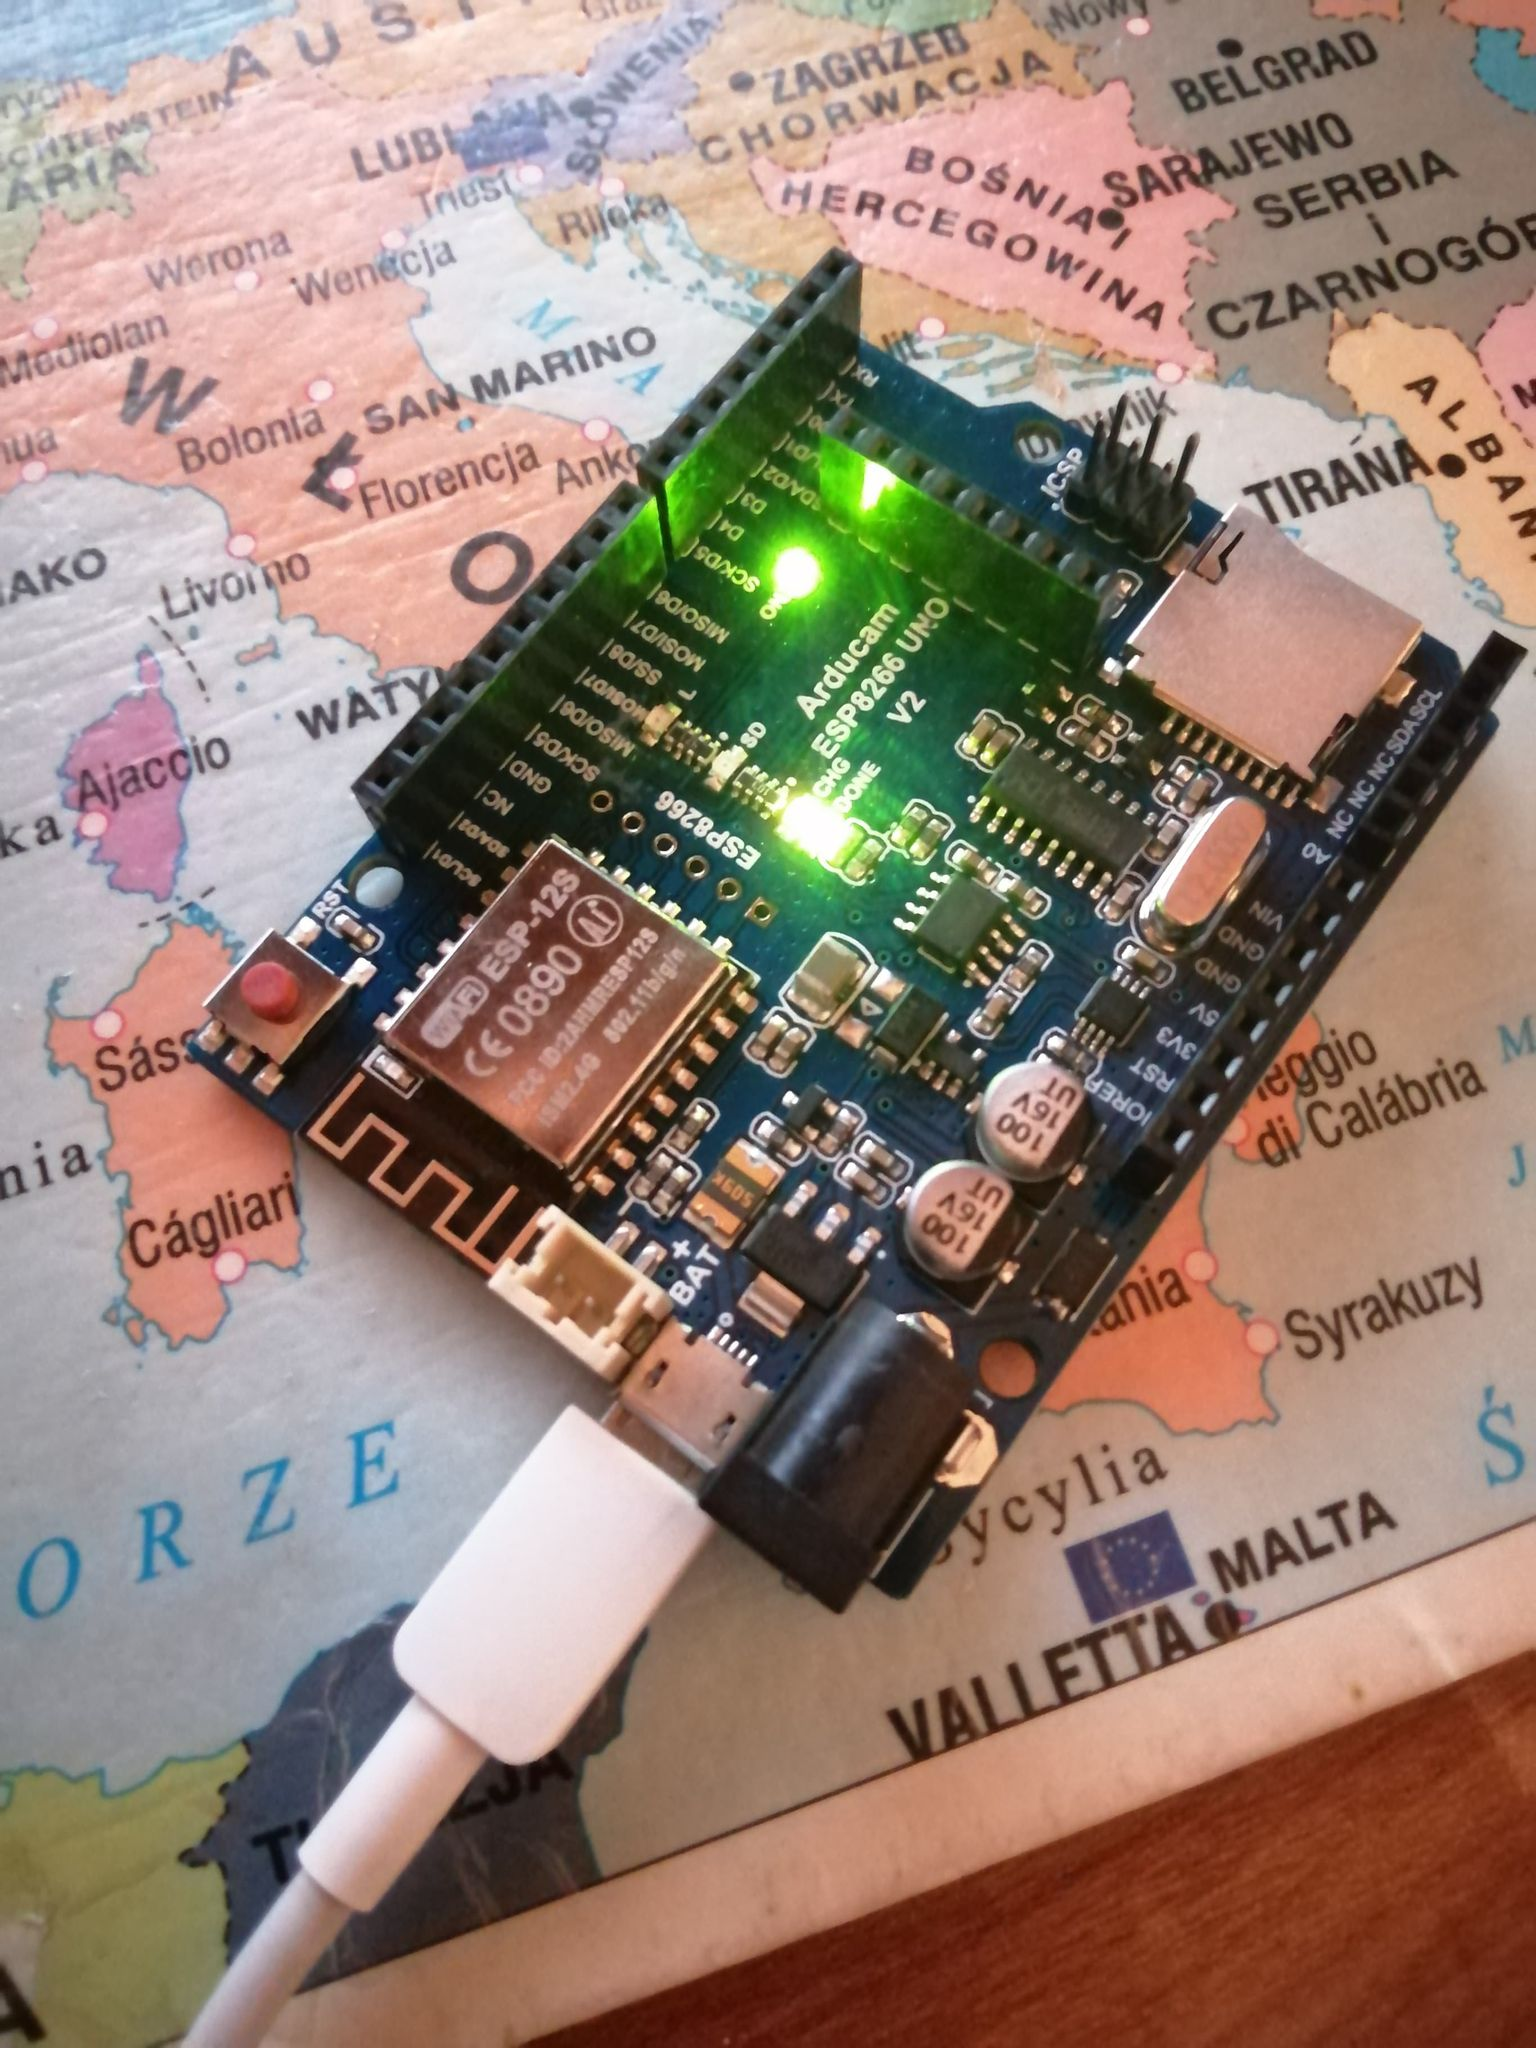
\includegraphics[width=5.0in]{arducam.jpg}
	\caption{arducam.\label{fig:arducam}}
\end{figure}


%%%%%%%%%%%%%%%%%%%%%%%%%%%%%%%%%%%%%%%%%%%%%%%%%%%%%%%%%%%%%%%%%
%% BIBLIOGRAPHY.
%%%%%%%%%%%%%%%%%%%%%%%%%%%%%%%%%%%%%%%%%%%%%%%%%%%%%%%%%%%%%%%%%

\clearpage
\phantomsection
\addcontentsline{toc}{chapter}{Bibliography}

\bibliographystyle{IEEEtran} % IEEE bibliographic/citation style.
\bibliography{IEEEfull,it-bib}

\end{document}


